\documentclass[11pt,aspectratio=43,ignorenonframetext,t]{beamer}
\usepackage[HTML]{xcolor}
% Presentation settings
\mode<presentation>{
  \usetheme[framenumber,titleframestart=1]{UoM_alex}
  \usefonttheme{professionalfonts} % using non standard fonts for beamer
  \usefonttheme{serif}             % set font to Arial
  \usepackage{fontspec}
  \setmainfont[Ligatures=TeX]{Arial}
}
\definecolor{uomlinkblue}{HTML}{0071BC}

% Handout settings
\mode<article>{
  \usepackage{fullpage}                  % use full page
  \usepackage{fontspec}                  % set font to Arial
    \setmainfont[Ligatures=TeX]{Arial}
  \setlength{\parskip}{1.5\baselineskip} % correct beamer line spacings
  \setlength{\parindent}{0cm}
  \usepackage{enumitem}
    \setlist[itemize]{topsep=0pt}
  % \definecolor{uomlinkblue}{HTML}{0071BC}
}


% Packages
\usepackage{graphicx}  % for graphics files
  \graphicspath{ {./images/png} }
\usepackage{amsmath}   % assumes amsmath package installed
  \allowdisplaybreaks[1] % allow eqnarrays to break across pages
\usepackage{amssymb}   % assumes amsmath package installed 
\usepackage{hyperref} % add hyperlinks to document. Settings are for accessiblity
  \hypersetup{
    colorlinks=true,
    linkcolor=uomlinkblue,
    filecolor=uomlinkblue,      
    urlcolor=uomlinkblue,
	pdflang={en-GB},
}
\usepackage[document]{ragged2e} % left aligned text for accessibility
% experimental - does fundamentally work, if with quite a bit of effort
%\usepackage{axessibility} % LaTeX readable equations for accessibility
%  \tagpdfsetup{tabsorder=structure,uncompress,activate-all,interwordspace=true}
%  \pdfextension catalog{/Lang (en-GB)}
%  \RequirePackage{luacode}
%  \directlua{require(axessibility.lua)}
\usepackage{tikz}
\usepackage{unicode-math} % unicode maths for accessibility
\usepackage{pdfcomment} % for alt text for accessibility
\usepackage{rotating}  % allow portrait figures and tables
\usepackage{subfigure} % allow matrices of figures
\usepackage{float}     % allows H option on floats to force here placement
\usepackage{multirow}  % allows merging of rows in tables
\usepackage{tabularx}  % allows fixed width tables
\usepackage{ctable}    % modifies \hline for use in table
\usepackage{bm}        % allow bold fonts in equations
\usepackage{pgf}       % allow graphics manipulation
\usepackage{media9}    % allow interactive flash files to be embedded
  \addmediapath{../media}
\usepackage{etoolbox}
  \makeatletter \preto{\@verbatim}{\topsep=0pt \partopsep=0pt} \makeatother  
  
% Custom commands
\newcommand{\matlab}{\emph{\sc{Matlab}}}
\newcommand{\maple}{\emph{\sc{Maple}}}
\newcommand{\simulink}{\emph{\sc{Simulink}}}
\newcommand{\dc}{d.c.}
\newcommand{\ac}{a.c.}
\newcommand{\rms}{RMS}
\newcommand{\wgn}{{\tt wgn}}
\newcommand{\sus}[1]{$^{\mbox{\scriptsize #1}}$}
\newcommand{\sub}[1]{$_{\mbox{\scriptsize #1}}$}
\newcommand{\chap}[1]{Chapter~\ref{#1}}
\newcommand{\sect}[1]{Section~\ref{#1}}
\newcommand{\fig}[1]{Fig.~\ref{#1}}
\newcommand{\tab}[1]{Table~\ref{#1}}
\newcommand{\equ}[1]{(\ref{#1})}
\newcommand{\appx}[1]{Appendix~\ref{#1}}
\newcommand{\degree}{\ensuremath{^\circ}}
\newcommand{\Vrms}{Vrms}
\newcommand{\Vpp}{V\sub{pp}}
\newcommand{\otoprule}{\midrule[\heavyrulewidth]}         
\newcolumntype{Z}{>{\centering\arraybackslash}X}  % tabularx centered columns 
\makeatletter \DeclareRobustCommand{\em}{\@nomath\em \if b\expandafter\@car\f@series\@nil \normalfont \else \bfseries \fi} \makeatother
\newcounter{example_number} % keep track of the example questions

\usepackage{hyperref}

%%%%%%%%%%%%%%%%%% FRONT MATTER %%%%%%%%%%%%%%%%%%
\title{Combinatorial Mesh Calculus (CMC): Lecture 4}
\author{Lectured by: \href{https://scholar.google.com/citations?user=x4R-snQAAAAJ&hl=en}{Dr. Kiprian Berbatov}$^1$\\
\smallskip
Lecture Notes Compiled by: \href{https://scholar.google.com/citations?user=CoIpITkAAAAJ&hl=en}{Muhammad Azeem}$^1$\\
\smallskip
Under the supervision of: \href{https://scholar.google.co.uk/citations?user=3nWJe5wAAAAJ&hl=en}{Prof. Andrey P. Jivkov}$^1$\\
\smallskip {\tiny $^1$Department of Mechanical and Aerospace Engineering, The University of Manchester, Oxford Road, Manchester M13 9PL, UK}
}
\date{\today}


\begin{document}

%========================= TITLE =========================
\begin{frame}
  \titlepage
  \begin{tikzpicture}[remember picture,overlay]
  \node[anchor=south east] at (current page.south east) {
    \href{https://youtube.com/@kipi.berbatov?si=gHtoBwWkTRCcCw2g}{
      \includegraphics[width=1.5cm]{youtube-icon.png}
    }
  };
\end{tikzpicture}
\end{frame}

% ============================================================
\section{Definition of an $R$–Module}
% ============================================================

\begin{frame}{Module over a Commutative Ring with Unity (CRWU)}
\begin{block}{Definition.}  
Let $R$ be a commutative ring with unity (CRWU), and let $(V, +, -, 0)$ be an abelian (commutative) group under addition.  
A \emph{scalar multiplication} $*: R\times V \to V$ makes $V$ an \textbf{$R$–module} if the following hold for all $\lambda,\mu\in R$ and $v,w\in V$:
\[
\begin{aligned}
(\lambda\mu)*v &= \lambda*(\mu*v) && \text{(Associativity of scalar mult.)}\\
(\lambda+\mu)*v &= \lambda*v+\mu*v && \text{(Distributivity over ring addition)}\\
\lambda*(v+w) &= \lambda*v+\lambda*w && \text{(Distributivity over module addition)}\\
1_R*v &= v && \text{(Unital condition)}
\end{aligned}
\]

\textbf{Notation:} $(V,+,*,0)$ is called an \emph{$R$–module}.  
If $R$ is a field, $V$ is a \textbf{vector space over $R$}.
    
\end{block}

\end{frame}

\begin{frame}[fragile]{Interpretation and Diagram}
\begin{block}{Idea}
Modules generalize vector spaces---where scalars come not from a field, but from a ring.

\begin{center}
\centering
\begin{tikzpicture}[
    node distance=2.5cm,
    every node/.style={inner sep=6pt}
]
    % 1. Define the nodes
    \node (R) at (0,0) {$R$};
    \node (V) at (2.5,0) {$V$};
    \node (RV) at (1.25,-1.2) {$R\times V$};
    \node (V2) at (2.5,-2.5) {$V$};
    
    % 2. Draw the arrows
    
    % R -> RV (Diagonal Left)
    \draw[->] (R) -- (RV); 
    
    % V -> RV (Diagonal Right)
    \draw[->] (V) -- (RV);

    % RV -> V2 (Labeled with action symbol)
    \draw[->] (RV) -- (V2) node[midway, right] {$*$};
    
    % Explanatory label at the bottom
    \node at (1.25,-3.2) {$(\lambda,v)\mapsto \lambda*v$};

\end{tikzpicture}
\end{center}

\end{block}
\end{frame}
% ============================================================
\section{Basic Examples}
% ============================================================

\begin{frame}{Examples of $R$–Modules}
Let $R$ be a CRWU, $m,n\in\mathbb{N}$.

\textbf{1. Coordinate Module:}  
\[
R^n = \{(a_1,\dots,a_n)\mid a_i\in R\}.
\]
Addition and scalar multiplication defined by
\[
(a_1,\dots,a_n)+(b_1,\dots,b_n)=(a_1+b_1,\dots,a_n+b_n),
\]
\[
\lambda*(a_1,\dots,a_n)=(\lambda a_1,\dots,\lambda a_n).
\]
Then $(R^n,+,*)$ is an $R$–module.  
When $R$ is a field, this is a vector space.

\textbf{2. Matrix Module:}  
\[
M_{m\times n}(R)=\{[a_{ij}]_{m\times n}\mid a_{ij}\in R\},
\]
with addition $(A+B)_{ij}=a_{ij}+b_{ij}$,  
and scalar multiplication $(\lambda A)_{ij}=\lambda a_{ij}$.
\end{frame}

\begin{frame}{Examples (continued)}
\begin{block}{}
\textbf{3. Zero Module:} $\{0\}$ with $r*0=0$ for all $r\in R$.  

\textbf{4. Free Module:}  
Let $S=\{e_1,\dots,e_n\}$ be a finite set.  
Define
\[
\mathrm{Free}_R(S) = \left\{ \sum_{i=1}^n \lambda_i e_i \mid \lambda_i\in R \right\}.
\]
Addition and scalar multiplication:
\[
\begin{aligned}
(\lambda_1 e_1+\dots+\lambda_n e_n) + (\mu_1 e_1+\dots+\mu_n e_n)
&= (\lambda_1+\mu_1)e_1+\dots+(\lambda_n+\mu_n)e_n,\\
r(\lambda_1 e_1+\dots+\lambda_n e_n)
&= (r\lambda_1)e_1+\dots+(r\lambda_n)e_n.
\end{aligned}
\]
Then $\mathrm{Free}_R(S)$ is an $R$–module.
\end{block}
\end{frame}

\begin{frame}{Free Module on Infinite Basis}
\begin{block}{}
    If $S$ is infinite, $\mathrm{Free}_R(S)$ consists of \textbf{finite linear combinations}:
\[
\lambda_1 e_{i_1}+\dots+\lambda_k e_{i_k}, \quad \lambda_i\in R.
\]
\textbf{Example:} $S=\{1,x,x^2,x^3,\dots\}$ then
\[
\mathrm{Free}_R(S)=R[x],
\]
the ring of polynomials over $R$—a free $R$–module with basis $$\{1,x,x^2,\dots\}$$.
\end{block}
\end{frame}

% ============================================================
\section{Linear Independence, Span, and Basis}
% ============================================================

\begin{frame}{Linear Independence and Span}
\vspace{-0.3cm}
\begin{block}{Definition: Let $V$ be an $R$–module, $e_1,\dots,e_n\in V$.}
\textbf{1. Linear Independence:}  
$\{e_1,\dots,e_n\}$ is linearly independent if
\[
\lambda_1 e_1+\dots+\lambda_n e_n=0 \Rightarrow \lambda_1=\dots=\lambda_n=0.
\]

\textbf{2. Linear Dependence:}  
The set is linearly dependent if there exist coefficients, not all zero, satisfying
\[
\lambda_1 e_1+\dots+\lambda_n e_n=0.
\]

\textbf{3. Span:}  
\vspace{-0.5cm}
\[
\mathrm{Span}_R\{e_1,\dots,e_n\}=\left\{\sum_{i=1}^n\lambda_i e_i\mid\lambda_i\in R\right\}.
\]

\textbf{4. Basis:}  
\vspace{-0.1cm}
A set $\{e_1,\dots,e_n\}$ is a basis of $V$ if it is linearly independent and spans $V$.
\end{block}
\end{frame}

\begin{frame}{Independence over $\mathbb{Z}$ and $\mathbb{Q}$}
\begin{block}{Example}
    Let $V=R^2$, $v_1=(2,0)$, $v_2=(3,0)$.
\begin{enumerate}
    \item$R=\mathbb{Q}$ (field). If $\lambda_1 v_1 + \lambda_2 v_2 = 0 \Rightarrow (2\lambda_1 + 3\lambda_2, 0)=0$. Thus $2\lambda_1+3\lambda_2=0 \Rightarrow \lambda_1=-\tfrac{3}{2}\lambda_2$.  
For independence we need both $\lambda_1=\lambda_2=0$. Hence $v_1,v_2$ are \textit{not} independent since nontrivial rational coefficients satisfy the equation.\
    \item $R=\mathbb{Z}$ (integral domain).  
$2\lambda_1+3\lambda_2=0$ implies $\lambda_1=-\tfrac{3}{2}\lambda_2$.  
But coefficients must be integers. The only integer solution is $\lambda_1=\lambda_2=0$.  
Hence $v_1,v_2$ are independent over $\mathbb{Z}$.
\end{enumerate}


\textbf{Conclusion:}  
Independence depends on the underlying ring.
\end{block}

\end{frame}

\begin{frame}{Failure of Division in General Modules}
\begin{block}{Remark}
If $R$ is a field and $\mu_1v_1+\dots+\mu_nv_n=0$ with $\mu_i\ne0$, then we can divide:
\[
v_i = \sum_{j\ne i} \frac{-\mu_j}{\mu_i} v_j.
\]
However, for general modules (where $R$ is not a field), division may not be possible, so such reduction cannot be performed.    
\end{block}

\end{frame}


\begin{frame}{Standard Basis of $R^n$}
\begin{block}{Example:}
    For $R^n$ define
\[
e_1=(1,0,\dots,0), \ e_2=(0,1,0,\dots,0), \ \dots, \ e_n=(0,\dots,0,1).
\]
\textbf{Claim:} $\{e_1,\dots,e_n\}$ is a basis of $R^n$.
\end{block}

\textbf{Proof:}
\begin{itemize}
  \item Every $v=(a_1,\dots,a_n)\in R^n$ can be written uniquely as
  \[
  v = a_1 e_1+\dots+a_n e_n.
  \]
  \item If $\sum \lambda_i e_i=0$, then all $\lambda_i=0$. Hence independence.
\end{itemize}
Therefore $\{e_i\}$ is a basis.
\end{frame}

\begin{frame}{Matrix Unit Basis of $M_{m\times n}(R)$}
\begin{block}{Example:}
For each $(i,j)$ define $E_{ij}\in M_{m\times n}(R)$ by
\[
(E_{ij})_{kl}=
\begin{cases}
1, & k=i,\ l=j,\\
0, & \text{otherwise}.
\end{cases}
\]
Then $\{E_{ij}\mid 1\le i\le m,1\le j\le n\}$ is a basis of $M_{m\times n}(R)$.
\end{block}
\textbf{Example (for $m=n=2$):}
\[
E_{11}=\begin{bmatrix}1&0\\0&0\end{bmatrix}, \quad
E_{12}=\begin{bmatrix}0&1\\0&0\end{bmatrix}, \quad
E_{21}=\begin{bmatrix}0&0\\1&0\end{bmatrix}, \quad
E_{22}=\begin{bmatrix}0&0\\0&1\end{bmatrix}.
\]
Any $A=\begin{bmatrix}a&b\\c&d\end{bmatrix}$ can be written as
\[
A = aE_{11}+bE_{12}+cE_{21}+dE_{22}.
\]
\end{frame}

\begin{frame}{Other Basis Examples}
\begin{block}{Zero Module:} $\phi$ is a basis of $\{0\}$.  
\end{block}
\begin{block}{Free Module:} If $S$ is a set, $S$ itself forms a basis of $\mathrm{Free}_R(S)$.  

\end{block}
\begin{block}{Polynomial Module:}  
For $S=\{1,x,x^2,\dots\}$,  
\[
R[x]=\mathrm{Free}_R(S)
\]
with basis $\{1,x,x^2,\dots\}$.
\end{block}


\end{frame}


\begin{frame}{Uniqueness of Representation}
\begin{block}{Proposition.}  
Let $R$ be a CRWU, $V$ an $R$–module, and $S=\{e_1,\dots,e_n\}\subseteq V$.  
Then $S$ is a basis of $V$ if and only if every $v\in V$ can be expressed uniquely as
\[
v=\lambda_1 e_1+\dots+\lambda_n e_n,\quad \lambda_i\in R.
\]  
\end{block}

\textbf{Proof.}
($\Rightarrow$)\\  
If $S$ is a basis, then by definition it spans $V$, so such $\lambda_i$ exist.  
Suppose $v=\sum \lambda_i e_i = \sum \mu_i e_i$. Then $\sum (\lambda_i-\mu_i)e_i=0$.  
Linear independence implies $\lambda_i-\mu_i=0$ for all $i$. Hence uniqueness.

($\Leftarrow$) \\ 
If every $v$ has a unique representation, then:\\
- Existence implies $S$ spans $V$.\\
- Uniqueness implies $S$ is linearly independent.  \\
Thus $S$ is a basis. $\square$
\end{frame}


\begin{frame}{Submodule}
\begin{block}{Definition.}  
Let $R$ be a CRWU, $V$ an $R$–module.  
A subset $W\subseteq V$ is called a \textbf{submodule} of $V$ if:
\begin{enumerate}
  \item $(W,+)$ is a subgroup of $(V,+)$,
  \item $\forall r\in R,\, w\in W:\, r*w\in W.$
\end{enumerate}

Equivalently, $W$ is a submodule iff
\[
\forall \lambda,\mu\in R,\ v,w\in W,\quad \lambda v+\mu w\in W.
\]
\end{block}
\end{frame}

\begin{frame}{Null Space and Image as Submodules}
Let $A\in M_{m\times n}(R)$.

\textbf{1. Null Space:}
\[
\mathrm{Null}(A)=\{x\in R^n\mid Ax=0_{R^m}\}.
\]
\textbf{Proof:}
If $x,y\in\mathrm{Null}(A)$ and $\lambda,\mu\in R$,
\[
A(\lambda x+\mu y)=\lambda A x+\mu A y=0.
\]
Hence closed under addition and scalar multiplication → submodule of $R^n$.

\textbf{2. Image:}
\[
\mathrm{Im}(A)=\{Ax\mid x\in R^n\}\subseteq R^m.
\]
If $y_1=Ax_1$, $y_2=Ax_2$, then for any $\lambda,\mu\in R$,
\[
\lambda y_1+\mu y_2=A(\lambda x_1+\mu x_2)\in \mathrm{Im}(A).
\]
Hence $\mathrm{Im}(A)$ is a submodule of $R^m$. $\square$
\end{frame}

\begin{frame}{Example with Numerical Matrix}
Let
\[
A=
\begin{bmatrix}
1 & 2 & 3\\
-2 & -4 & -8
\end{bmatrix}\in M_{2\times 3}(\mathbb{Q}).
\]

\textbf{Find } $\mathrm{Null}(A)$:
\[
A x = 0 \Rightarrow
\begin{cases}
x_1+2x_2+3x_3=0,\\
-2x_1-4x_2-8x_3=0.
\end{cases}
\]
Second equation is $-2\times$ first, redundant.  
Solve first:
\[
x_1=-2x_2-3x_3.
\]
Hence
\[
x=(x_1,x_2,x_3)=x_2(-2,1,0)+x_3(-3,0,1).
\]
Therefore
\[
\mathrm{Null}(A)=\mathrm{Span}_{\mathbb{Q}}\{(-2,1,0),(-3,0,1)\}.
\]
\end{frame}

\begin{frame}{Image of the Same Matrix (continued)}
\[
\mathrm{Im}(A)=\mathrm{Span}_{\mathbb{Q}}
\left\{
\begin{bmatrix}1\\-2\end{bmatrix},
\begin{bmatrix}2\\-4\end{bmatrix},
\begin{bmatrix}3\\-8\end{bmatrix}
\right\}.
\]
Notice that
\[
\begin{bmatrix}2\\-4\end{bmatrix}=2\begin{bmatrix}1\\-2\end{bmatrix}, \qquad
\begin{bmatrix}3\\-8\end{bmatrix}=3\begin{bmatrix}1\\-2\end{bmatrix}
+\begin{bmatrix}0\\-2\end{bmatrix},
\]
so only one of these is independent.  
Therefore,
\[
\mathrm{Im}(A)=\mathrm{Span}_{\mathbb{Q}}
\left\{
\begin{bmatrix}1\\-2\end{bmatrix}
\right\}.
\]
Hence
\[
\dim_{\mathbb{Q}}(\mathrm{Im}(A))=1,\quad
\dim_{\mathbb{Q}}(\mathrm{Null}(A))=2.
\]

\textbf{Observation (Rank–Nullity analogue):}
\[
\dim_{\mathbb{Q}}(\mathrm{Im}(A))+\dim_{\mathbb{Q}}(\mathrm{Null}(A))=3=\text{number of columns}.
\]
\end{frame}


\begin{frame}[fragile]{Submodules as Linear Substructures}

\begin{center}
\centering
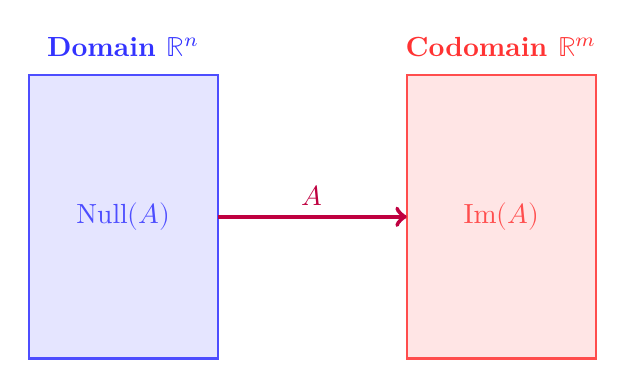
\begin{tikzpicture}[scale=1.2] % Kept scale, removed >=Stealth
% Domain space
\draw[thick, blue!70, fill=blue!10] (-2,-1.5) rectangle (0,1.5);
\node[blue!80, font=\bfseries] at (-1,1.8) {Domain $\mathbb{R}^n$};
\node[blue!70] at (-1,0) {Null$(A)$};

% Codomain space
\draw[thick, red!70, fill=red!10] (2,-1.5) rectangle (4,1.5);
\node[red!80, font=\bfseries] at (3,1.8) {Codomain $\mathbb{R}^m$};
\node[red!70] at (3,0) {Im$(A)$};

% Mapping arrow
\draw[->, ultra thick, purple] (0,0) -- node[above] {$A$} (2,0);
\end{tikzpicture}
\end{center}

\vspace{0.3cm}

\textbf{Interpretation:}  
\begin{itemize}
\item Null$(A)$ lives in the domain $R^n$ (vectors mapped to zero)
\item Im$(A)$ lives in the codomain $R^m$ (all possible outputs)
\item Each is a submodule closed under addition and scalar multiplication
\end{itemize}

\end{frame}


\begin{frame}{Remarks and Extensions}
\begin{itemize}
  \item Every vector space is a module, but not every module is a vector space (lack of division in $R$).
  \item Submodules play the same role as subspaces.
  \item The null and image submodules generalize the kernel and image of a linear map.
  \item Free modules generalize coordinate spaces $R^n$.
  \item If $R$ is a principal ideal domain, many results from linear algebra (rank, basis, independence) extend naturally.
\end{itemize}

\textbf{Important note:}  
Modules over non-fields can have surprising behaviors — e.g., not every submodule has a complement, not every module has a basis.
\end{frame}


\begin{frame}{Summary of Lecture 4}
\begin{itemize}
  \item Defined an $R$–module as an abelian group with a compatible scalar multiplication.
  \item Showed that for a CRWU, $R^n$, $M_{m\times n}(R)$, and $R[x]$ are $R$–modules.
  \item Introduced \textbf{linear independence}, \textbf{span}, and \textbf{basis} in modules.
  \item Proved characterization: $S$ is a basis $\iff$ each $v$ has a unique expression.
  \item Defined submodules and proved closure criterion $\lambda v+\mu w\in W$.
  \item Proved that $\mathrm{Null}(A)$ and $\mathrm{Im}(A)$ are submodules.
  \item Worked out complete example for $A\in M_{2\times3}(\mathbb{Q})$, computing both $\mathrm{Null}(A)$ and $\mathrm{Im}(A)$.
\end{itemize}
\end{frame}

\begin{frame}{Thanks}
    \begin{figure}
        \centering
        \includegraphics[width=0.85\linewidth]{Thanks.png}
    \end{figure}
\end{frame}

\end{document}
